\documentclass[twoside]{book}

% Packages required by doxygen
\usepackage{fixltx2e}
\usepackage{calc}
\usepackage{doxygen}
\usepackage[export]{adjustbox} % also loads graphicx
\usepackage{graphicx}
\usepackage[utf8]{inputenc}
\usepackage{makeidx}
\usepackage{multicol}
\usepackage{multirow}
\PassOptionsToPackage{warn}{textcomp}
\usepackage{textcomp}
\usepackage[nointegrals]{wasysym}
\usepackage[table]{xcolor}

% Font selection
\usepackage[T1]{fontenc}
\usepackage[scaled=.90]{helvet}
\usepackage{courier}
\usepackage{amssymb}
\usepackage{sectsty}
\renewcommand{\familydefault}{\sfdefault}
\allsectionsfont{%
  \fontseries{bc}\selectfont%
  \color{darkgray}%
}
\renewcommand{\DoxyLabelFont}{%
  \fontseries{bc}\selectfont%
  \color{darkgray}%
}
\newcommand{\+}{\discretionary{\mbox{\scriptsize$\hookleftarrow$}}{}{}}

% Page & text layout
\usepackage{geometry}
\geometry{%
  a4paper,%
  top=2.5cm,%
  bottom=2.5cm,%
  left=2.5cm,%
  right=2.5cm%
}
\tolerance=750
\hfuzz=15pt
\hbadness=750
\setlength{\emergencystretch}{15pt}
\setlength{\parindent}{0cm}
\setlength{\parskip}{3ex plus 2ex minus 2ex}
\makeatletter
\renewcommand{\paragraph}{%
  \@startsection{paragraph}{4}{0ex}{-1.0ex}{1.0ex}{%
    \normalfont\normalsize\bfseries\SS@parafont%
  }%
}
\renewcommand{\subparagraph}{%
  \@startsection{subparagraph}{5}{0ex}{-1.0ex}{1.0ex}{%
    \normalfont\normalsize\bfseries\SS@subparafont%
  }%
}
\makeatother

% Headers & footers
\usepackage{fancyhdr}
\pagestyle{fancyplain}
\fancyhead[LE]{\fancyplain{}{\bfseries\thepage}}
\fancyhead[CE]{\fancyplain{}{}}
\fancyhead[RE]{\fancyplain{}{\bfseries\leftmark}}
\fancyhead[LO]{\fancyplain{}{\bfseries\rightmark}}
\fancyhead[CO]{\fancyplain{}{}}
\fancyhead[RO]{\fancyplain{}{\bfseries\thepage}}
\fancyfoot[LE]{\fancyplain{}{}}
\fancyfoot[CE]{\fancyplain{}{}}
\fancyfoot[RE]{\fancyplain{}{\bfseries\scriptsize Generated by Doxygen }}
\fancyfoot[LO]{\fancyplain{}{\bfseries\scriptsize Generated by Doxygen }}
\fancyfoot[CO]{\fancyplain{}{}}
\fancyfoot[RO]{\fancyplain{}{}}
\renewcommand{\footrulewidth}{0.4pt}
\renewcommand{\chaptermark}[1]{%
  \markboth{#1}{}%
}
\renewcommand{\sectionmark}[1]{%
  \markright{\thesection\ #1}%
}

% Indices & bibliography
\usepackage{natbib}
\usepackage[titles]{tocloft}
\setcounter{tocdepth}{3}
\setcounter{secnumdepth}{5}
\makeindex

% Hyperlinks (required, but should be loaded last)
\usepackage{ifpdf}
\ifpdf
  \usepackage[pdftex,pagebackref=true]{hyperref}
\else
  \usepackage[ps2pdf,pagebackref=true]{hyperref}
\fi
\hypersetup{%
  colorlinks=true,%
  linkcolor=blue,%
  citecolor=blue,%
  unicode%
}

% Custom commands
\newcommand{\clearemptydoublepage}{%
  \newpage{\pagestyle{empty}\cleardoublepage}%
}

\usepackage{caption}
\captionsetup{labelsep=space,justification=centering,font={bf},singlelinecheck=off,skip=4pt,position=top}

%===== C O N T E N T S =====

\begin{document}

% Titlepage & ToC
\hypersetup{pageanchor=false,
             bookmarksnumbered=true,
             pdfencoding=unicode
            }
\pagenumbering{alph}
\begin{titlepage}
\vspace*{7cm}
\begin{center}%
{\Large My Project }\\
\vspace*{1cm}
{\large Generated by Doxygen 1.8.12}\\
\end{center}
\end{titlepage}
\clearemptydoublepage
\pagenumbering{roman}
\tableofcontents
\clearemptydoublepage
\pagenumbering{arabic}
\hypersetup{pageanchor=true}

%--- Begin generated contents ---
\chapter{Namespace Index}
\section{Namespace List}
Here is a list of all documented namespaces with brief descriptions\+:\begin{DoxyCompactList}
\item\contentsline{section}{\hyperlink{namespace_windows_service1}{Windows\+Service1} }{\pageref{namespace_windows_service1}}{}
\end{DoxyCompactList}

\chapter{Hierarchical Index}
\section{Class Hierarchy}
This inheritance list is sorted roughly, but not completely, alphabetically\+:\begin{DoxyCompactList}
\item Installer\begin{DoxyCompactList}
\item \contentsline{section}{Windows\+Service1.\+Installer1}{\pageref{class_windows_service1_1_1_installer1}}{}
\end{DoxyCompactList}
\item Service\+Base\begin{DoxyCompactList}
\item \contentsline{section}{Windows\+Service1.\+Service1}{\pageref{class_windows_service1_1_1_service1}}{}
\end{DoxyCompactList}
\item \contentsline{section}{Serv\+Lisener}{\pageref{class_serv_lisener}}{}
\item \contentsline{section}{Windows\+Service1.\+Serv\+Lisener}{\pageref{class_windows_service1_1_1_serv_lisener}}{}
\item \contentsline{section}{Windows\+Service1.\+Translator}{\pageref{class_windows_service1_1_1_translator}}{}
\end{DoxyCompactList}

\chapter{Class Index}
\section{Class List}
Here are the classes, structs, unions and interfaces with brief descriptions\+:\begin{DoxyCompactList}
\item\contentsline{section}{\hyperlink{class_windows_service1_1_1_installer1}{Windows\+Service1.\+Installer1} }{\pageref{class_windows_service1_1_1_installer1}}{}
\item\contentsline{section}{\hyperlink{class_windows_service1_1_1_service1}{Windows\+Service1.\+Service1} }{\pageref{class_windows_service1_1_1_service1}}{}
\item\contentsline{section}{\hyperlink{class_serv_lisener}{Serv\+Lisener} \\*Класс поддерживающий соединение }{\pageref{class_serv_lisener}}{}
\item\contentsline{section}{\hyperlink{class_windows_service1_1_1_serv_lisener}{Windows\+Service1.\+Serv\+Lisener} }{\pageref{class_windows_service1_1_1_serv_lisener}}{}
\item\contentsline{section}{\hyperlink{class_windows_service1_1_1_translator}{Windows\+Service1.\+Translator} }{\pageref{class_windows_service1_1_1_translator}}{}
\end{DoxyCompactList}

\chapter{File Index}
\section{File List}
Here is a list of all documented files with brief descriptions\+:\begin{DoxyCompactList}
\item\contentsline{section}{\hyperlink{_class1_8cs}{Class1.\+cs} }{\pageref{_class1_8cs}}{}
\end{DoxyCompactList}

\chapter{Namespace Documentation}
\hypertarget{namespace_windows_service1}{}\section{Windows\+Service1 Namespace Reference}
\label{namespace_windows_service1}\index{Windows\+Service1@{Windows\+Service1}}
\subsection*{Classes}
\begin{DoxyCompactItemize}
\item 
class \hyperlink{class_windows_service1_1_1_installer1}{Installer1}
\item 
class {\bfseries Program}
\item 
class \hyperlink{class_windows_service1_1_1_service1}{Service1}
\item 
class \hyperlink{class_windows_service1_1_1_serv_lisener}{Serv\+Lisener}
\item 
class \hyperlink{class_windows_service1_1_1_translator}{Translator}
\end{DoxyCompactItemize}

\chapter{Class Documentation}
\hypertarget{class_windows_service1_1_1_installer1}{}\section{Windows\+Service1.\+Installer1 Class Reference}
\label{class_windows_service1_1_1_installer1}\index{Windows\+Service1.\+Installer1@{Windows\+Service1.\+Installer1}}
Inheritance diagram for Windows\+Service1.\+Installer1\+:\begin{figure}[H]
\begin{center}
\leavevmode
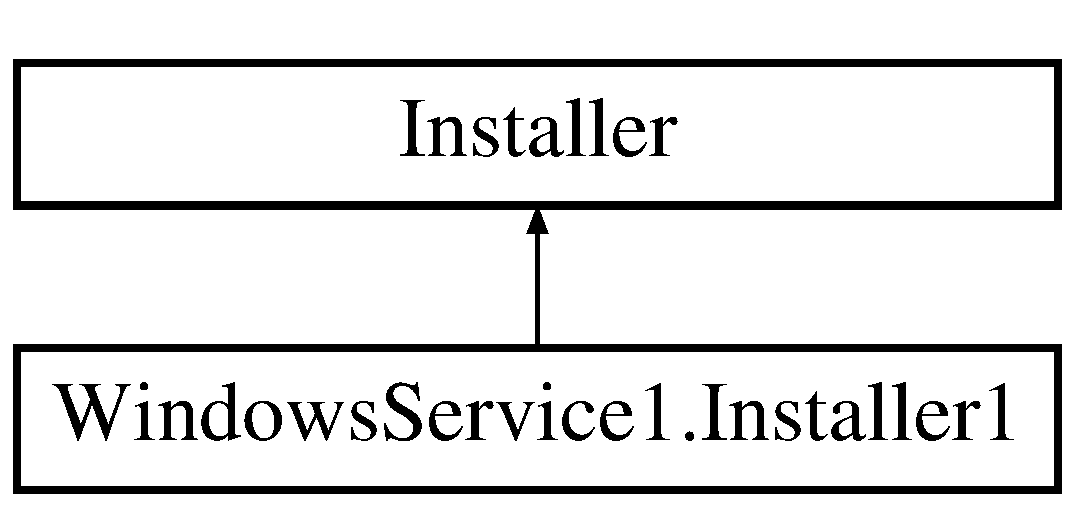
\includegraphics[height=2.000000cm]{class_windows_service1_1_1_installer1}
\end{center}
\end{figure}
\subsection*{Protected Member Functions}
\begin{DoxyCompactItemize}
\item 
override void \hyperlink{class_windows_service1_1_1_installer1_a77b7ef72d1485157054985463d92f70e}{Dispose} (bool disposing)
\begin{DoxyCompactList}\small\item\em Освободить все используемые ресурсы. \end{DoxyCompactList}\end{DoxyCompactItemize}


\subsection{Member Function Documentation}
\hypertarget{class_windows_service1_1_1_installer1_a77b7ef72d1485157054985463d92f70e}{}\label{class_windows_service1_1_1_installer1_a77b7ef72d1485157054985463d92f70e} 
\index{Windows\+Service1\+::\+Installer1@{Windows\+Service1\+::\+Installer1}!Dispose@{Dispose}}
\index{Dispose@{Dispose}!Windows\+Service1\+::\+Installer1@{Windows\+Service1\+::\+Installer1}}
\subsubsection{\texorpdfstring{Dispose()}{Dispose()}}
{\footnotesize\ttfamily override void Windows\+Service1.\+Installer1.\+Dispose (\begin{DoxyParamCaption}\item[{bool}]{disposing }\end{DoxyParamCaption})\hspace{0.3cm}{\ttfamily [inline]}, {\ttfamily [protected]}}



Освободить все используемые ресурсы. 


\begin{DoxyParams}{Parameters}
{\em disposing} & истинно, если управляемый ресурс должен быть удален; иначе ложно.\\
\hline
\end{DoxyParams}


The documentation for this class was generated from the following files\+:\begin{DoxyCompactItemize}
\item 
Installer1.\+cs\item 
Installer1.\+Designer.\+cs\end{DoxyCompactItemize}

\hypertarget{class_windows_service1_1_1_service1}{}\section{Windows\+Service1.\+Service1 Class Reference}
\label{class_windows_service1_1_1_service1}\index{Windows\+Service1.\+Service1@{Windows\+Service1.\+Service1}}
Inheritance diagram for Windows\+Service1.\+Service1\+:\begin{figure}[H]
\begin{center}
\leavevmode
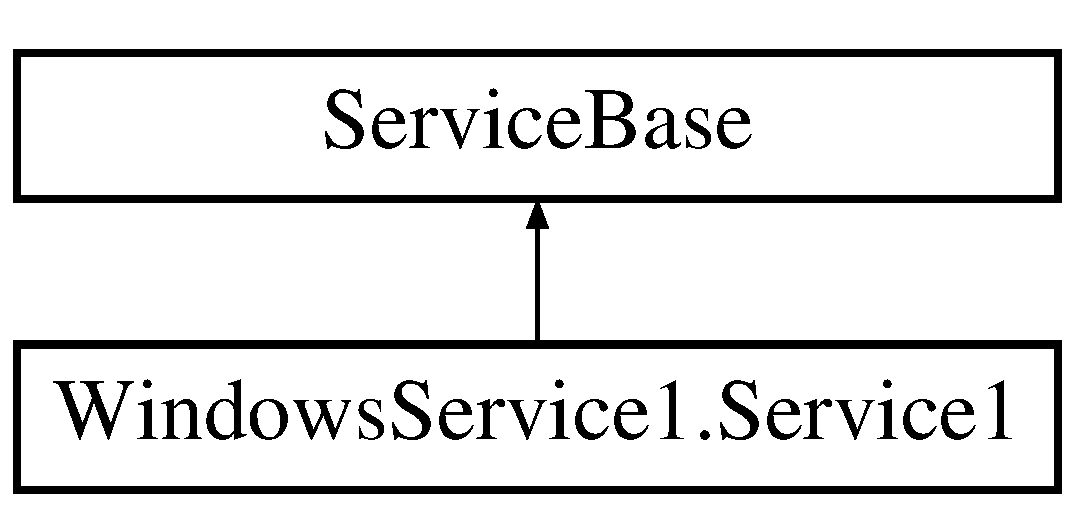
\includegraphics[height=2.000000cm]{class_windows_service1_1_1_service1}
\end{center}
\end{figure}
\subsection*{Protected Member Functions}
\begin{DoxyCompactItemize}
\item 
\hypertarget{class_windows_service1_1_1_service1_a625f720f2cd425cf8e90ec7432947ef9}{}\label{class_windows_service1_1_1_service1_a625f720f2cd425cf8e90ec7432947ef9} 
override void {\bfseries On\+Start} (string\mbox{[}$\,$\mbox{]} args)
\item 
\hypertarget{class_windows_service1_1_1_service1_ab9ac7ce457cd629619ef63dd097cae38}{}\label{class_windows_service1_1_1_service1_ab9ac7ce457cd629619ef63dd097cae38} 
override void {\bfseries On\+Continue} ()
\item 
\hypertarget{class_windows_service1_1_1_service1_a7fece590f3df413de51dde388a241314}{}\label{class_windows_service1_1_1_service1_a7fece590f3df413de51dde388a241314} 
override void {\bfseries On\+Pause} ()
\item 
\hypertarget{class_windows_service1_1_1_service1_ae5e4fb04766a3a46b4a93a3bc868b034}{}\label{class_windows_service1_1_1_service1_ae5e4fb04766a3a46b4a93a3bc868b034} 
override void {\bfseries On\+Stop} ()
\item 
override void \hyperlink{class_windows_service1_1_1_service1_ae10ffc85ffbeade32c0c40756c334c73}{Dispose} (bool disposing)
\begin{DoxyCompactList}\small\item\em Освободить все используемые ресурсы. \end{DoxyCompactList}\end{DoxyCompactItemize}


\subsection{Member Function Documentation}
\hypertarget{class_windows_service1_1_1_service1_ae10ffc85ffbeade32c0c40756c334c73}{}\label{class_windows_service1_1_1_service1_ae10ffc85ffbeade32c0c40756c334c73} 
\index{Windows\+Service1\+::\+Service1@{Windows\+Service1\+::\+Service1}!Dispose@{Dispose}}
\index{Dispose@{Dispose}!Windows\+Service1\+::\+Service1@{Windows\+Service1\+::\+Service1}}
\subsubsection{\texorpdfstring{Dispose()}{Dispose()}}
{\footnotesize\ttfamily override void Windows\+Service1.\+Service1.\+Dispose (\begin{DoxyParamCaption}\item[{bool}]{disposing }\end{DoxyParamCaption})\hspace{0.3cm}{\ttfamily [inline]}, {\ttfamily [protected]}}



Освободить все используемые ресурсы. 


\begin{DoxyParams}{Parameters}
{\em disposing} & истинно, если управляемый ресурс должен быть удален; иначе ложно.\\
\hline
\end{DoxyParams}


The documentation for this class was generated from the following files\+:\begin{DoxyCompactItemize}
\item 
Service1.\+cs\item 
Service1.\+Designer.\+cs\end{DoxyCompactItemize}

\hypertarget{class_serv_lisener}{}\section{Serv\+Lisener Class Reference}
\label{class_serv_lisener}\index{Serv\+Lisener@{Serv\+Lisener}}


Класс поддерживающий соединение  




\subsection{Detailed Description}
Класс поддерживающий соединение 

\begin{DoxyAuthor}{Author}
No\+Random 
\end{DoxyAuthor}
\begin{DoxyDate}{Date}
24 дек. 2016 г ! 
\end{DoxyDate}


The documentation for this class was generated from the following file\+:\begin{DoxyCompactItemize}
\item 
\hyperlink{_class1_8cs}{Class1.\+cs}\end{DoxyCompactItemize}

\hypertarget{class_windows_service1_1_1_serv_lisener}{}\section{Windows\+Service1.\+Serv\+Lisener Class Reference}
\label{class_windows_service1_1_1_serv_lisener}\index{Windows\+Service1.\+Serv\+Lisener@{Windows\+Service1.\+Serv\+Lisener}}
\subsection*{Public Member Functions}
\begin{DoxyCompactItemize}
\item 
\hypertarget{class_windows_service1_1_1_serv_lisener_aee4569298b222b1eb1b585a86b6d60fe}{}\label{class_windows_service1_1_1_serv_lisener_aee4569298b222b1eb1b585a86b6d60fe} 
void {\bfseries start} ()
\item 
\hypertarget{class_windows_service1_1_1_serv_lisener_a0f19c3cf63fa857170e0f49b8bd450d8}{}\label{class_windows_service1_1_1_serv_lisener_a0f19c3cf63fa857170e0f49b8bd450d8} 
void {\bfseries stop} ()
\end{DoxyCompactItemize}
\subsection*{Public Attributes}
\begin{DoxyCompactItemize}
\item 
\hypertarget{class_windows_service1_1_1_serv_lisener_abbc0fe7c48c7b0903d9cdf21efe50d4a}{}\label{class_windows_service1_1_1_serv_lisener_abbc0fe7c48c7b0903d9cdf21efe50d4a} 
Tcp\+Listener {\bfseries tcp\+Server}
\end{DoxyCompactItemize}


The documentation for this class was generated from the following file\+:\begin{DoxyCompactItemize}
\item 
\hyperlink{_class1_8cs}{Class1.\+cs}\end{DoxyCompactItemize}

\hypertarget{class_windows_service1_1_1_translator}{}\section{Windows\+Service1.\+Translator Class Reference}
\label{class_windows_service1_1_1_translator}\index{Windows\+Service1.\+Translator@{Windows\+Service1.\+Translator}}
\subsection*{Public Member Functions}
\begin{DoxyCompactItemize}
\item 
\hypertarget{class_windows_service1_1_1_translator_a8681ee41bba871f018b8e6183d9f487f}{}\label{class_windows_service1_1_1_translator_a8681ee41bba871f018b8e6183d9f487f} 
{\bfseries Translator} (string i, string o)
\item 
\hypertarget{class_windows_service1_1_1_translator_a1915c8b70d07c0f9fe34f8ebb9ff64ae}{}\label{class_windows_service1_1_1_translator_a1915c8b70d07c0f9fe34f8ebb9ff64ae} 
string {\bfseries Perevod} (string text)
\end{DoxyCompactItemize}


The documentation for this class was generated from the following file\+:\begin{DoxyCompactItemize}
\item 
\hyperlink{_class1_8cs}{Class1.\+cs}\end{DoxyCompactItemize}

\chapter{File Documentation}
\hypertarget{_class1_8cs}{}\section{Class1.\+cs File Reference}
\label{_class1_8cs}\index{Class1.\+cs@{Class1.\+cs}}
\subsection*{Classes}
\begin{DoxyCompactItemize}
\item 
class \hyperlink{class_windows_service1_1_1_serv_lisener}{Windows\+Service1.\+Serv\+Lisener}
\item 
class \hyperlink{class_windows_service1_1_1_translator}{Windows\+Service1.\+Translator}
\end{DoxyCompactItemize}
\subsection*{Namespaces}
\begin{DoxyCompactItemize}
\end{DoxyCompactItemize}

%--- End generated contents ---

% Index
\backmatter
\newpage
\phantomsection
\clearemptydoublepage
\addcontentsline{toc}{chapter}{Index}
\printindex

\end{document}
